\chapter{Introduction}

\section{Background on Robosub}

\subsection{Information about the competition}
Robosub is an international AUV competition where students from around the world build their own customized AUV to complete a series of underwater missions that involve both visual tasks and acoustics task. The competition is held annually in TRANSDEC (Transducer Evaluation Center) man-made pool.

\begin{figure}[ht]
\centering

        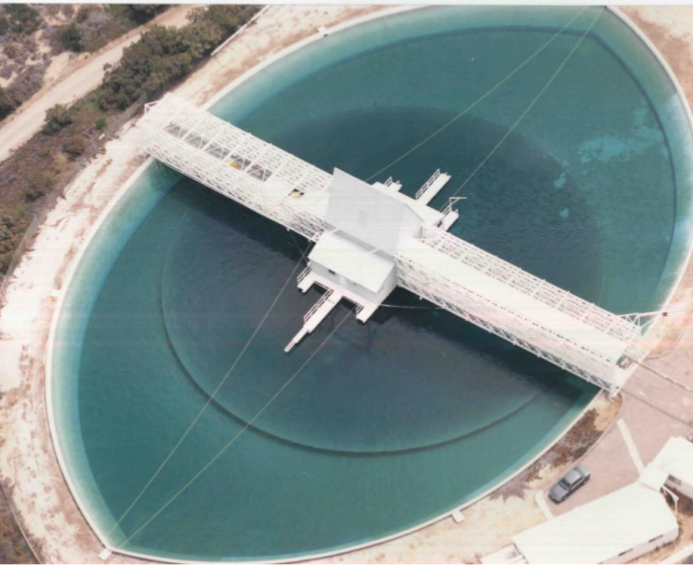
\includegraphics[width=0.8\textwidth, height=0.3\textheight]{transdec_aerial.png}
        \caption{Aerial view of TRANSDEC. Operational depth of 16 ft for most vision tasks}
        \label{fig:transdec_aerial}

\end{figure}

\subsection{Description of vision tasks}
Vision tasks in Robosub can divided into forward-facing tasks and bottom-facing tasks which poses different sets of challenges. Since the tasks do not vary significantly every year, we can use datasets collected from this year's competition as testbed for our vision algorithms.

\begin{figure}[ht]
\centering

        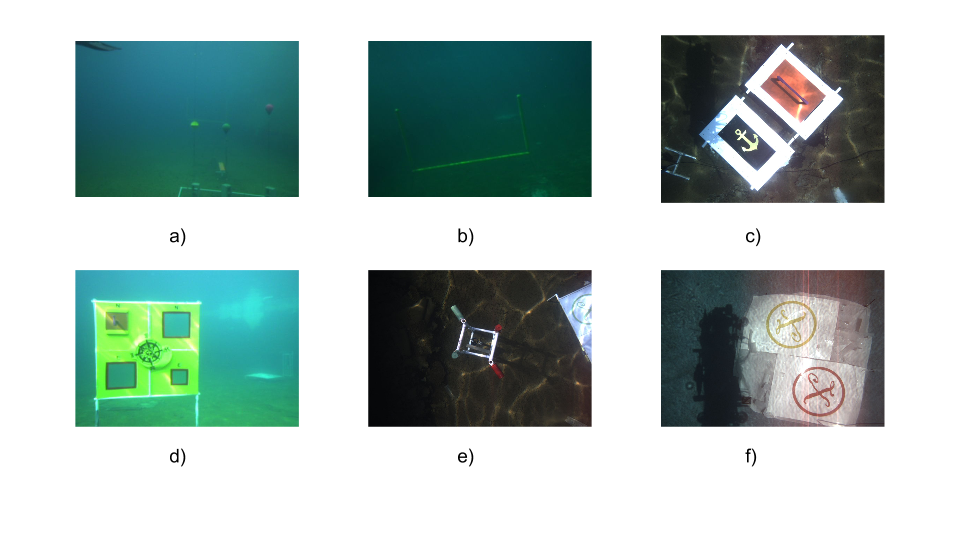
\includegraphics[width=0.8\textwidth, height=0.3\textheight]{robosub_vision_tasks.png}
        \caption{Robosub 2016 Vision Tasks. a) Scuttle Ship b) Navigate Channel c) Weigh Anchor d) Set Course e) Bury Treasure (Coins) f) Bury Treasure (Island)}
        \label{fig:robosub2016_tasks}

\end{figure}

\begin{enumerate}
    \item \textbf{Scuttle Ship (Buoy)}
        A recurring task where the AUV has identify the correct color buoy and touch it. There are two major challenges with this task:
        \begin{enumerate}[labels=(\alph*)]
        \item Red buoy tends to exhibit color distortion as red wavelength attenuates the fastest \cite{Galdran2015}.
        \item Non-uniform illumination on top-half of buoys make it hard to distinguish the buoys.
        \end{enumerate}
    \item \textbf{Navigate Channel} \\
        The AUV is required to move in between and over the PVC pipes.
    \item \textbf{Weight Anchor} \\
        Classic object classification task where the AUV is required to drop a marker into the correct bin to obtain maximum points after removing the cover using a manipulator.
    \item \textbf{Set Course} \\
        Identification of covered square (orange panel) and remove it. Fire two markers over 2 smaller holes. As yellow and orange are really close on the colour spectrum, this forces us to use other visual cues such as edge for better detection.
    \item \textbf{Bury Treasure} \\
        For this task, one has to identify the small cylinders (red and green) and drop them onto their respective colored circles (on the Island). Identifying and distinguishing small objects afar (4 m) underwater is the biggest challenge in this task. Besides that, the dropped cylinders may potentially occlude the circles.
\end{enumerate}

\section{Challenges in Underwater Image Processing}

Many literature such as \outcite{M2016} that investigates various underwater image restoration methods cite haze formation which happens as light propagated from object undergoes attenuation and scattering causing image with low contrast. In addition, Beer-Lambert law \cite{gevers2012color} states relates attenuation of light to properties of water medium; therefore, light components with low wavelength; green and blue are not as easily absorbed compared to red wavelength. This causes underwater images tend to have greenish or bluish color cast.

\begin{figure}[ht]
\centering

        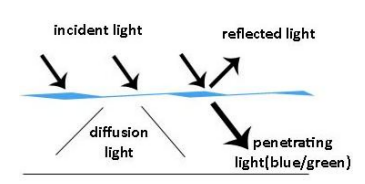
\includegraphics[width=0.8\textwidth, height=0.2\textheight]{underwater_beerlambert.png}
        \caption{Absorption of light at the surface}
        \label{fig:water_surface_effect}

\end{figure}

\section{Project Requirements Analysis}
Though it is the objective of the project to design a vision framework for the Robosub missions, the vision framework should also be easily extended to work for more complex real world applications. 

\subsection{Nature of tasks}
\begin{enumerate}
    \item Vision algorithms perform with acceptable accuracy under the following conditions:
    \begin{figure}[ht]
    \centering
            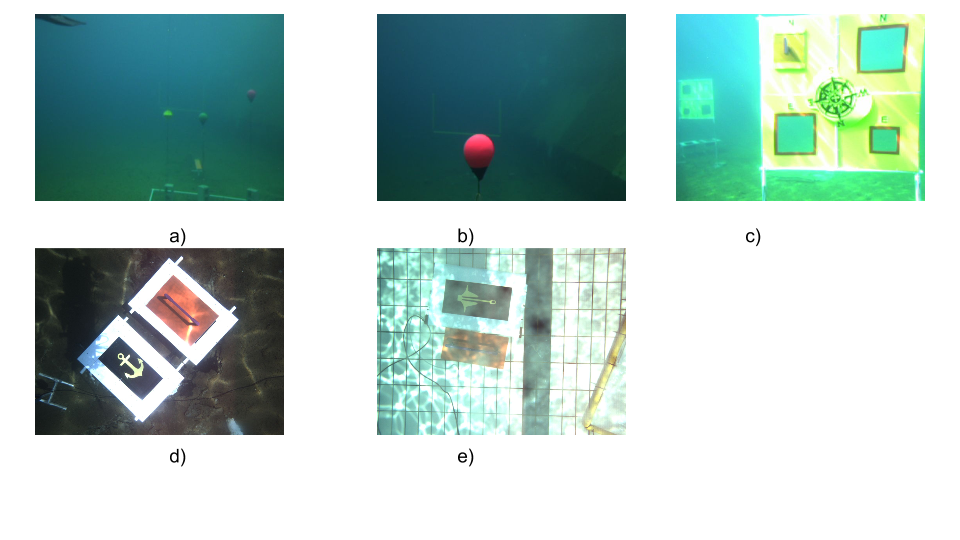
\includegraphics[width=0.8\textwidth, height=0.3\textheight]{task_challenges.png}
            \caption{Different vision challenges. a) Haze formation b) Partial occlusion c) Non-uniform illumination d) Sunlight flickers e) Shadow}
            \label{fig:vision_challenges}
    \end{figure}
    \item Low detection latency (near real-time) \\
        AUV needs to make swift decision based on sensor inputs to complete task under time constraints (same for real world time critical mission i.e underwater mine detection)
    \item Geometric properties of objects are made known in advance
    \item Short-period single target tracking for  task (unlike video surveillance application)
    \item Able to detect objects from far away (5m) and near distance (for manipulation task)
\end{enumerate}